% Provenance (never printed): cycle 3 / 6e "La planete Terre, l'environnement
% et l'action humaine" (the Earth in the Solar System; conditions for life);
% see sources/book1/PROVENANCE.md. Book 1, grade 6, chapter 1.
\chapter{地球，太阳系中的一颗行星}\label{ch:g6:earth-a-planet}

三个机器人探测器已被送入太空。它们一个接一个地
传回一张图片，像明信片一样。第一张来自金星：一个苍白的球体，
被厚厚的\omterm{def:g4:clouds-rain-snow:cloud}{云层}包裹，那里热得足以熔化铅，空气
以令人窒息的重量压在地面上。第二张来自火星：
一片红色、寒冷、尘土飞扬的\omterm{def:g5:weather-and-climate:desert}{沙漠}，天空稀薄。第三个探测器把镜头
转回了家园：一个蓝白色的球体，有\omterm{def:g2:water-on-earth:ocean}{海洋}、\omterm{def:g4:clouds-rain-snow:cloud}{云层}和
冰雪。三颗行星，同绕一颗太阳，彼此为邻。为何其中
只有一颗呈蓝色？
% ledger: nasa:venus-clouds, nasa:mars-water

\begin{omfigure}
\begin{minipage}[t]{0.31\linewidth}\centering
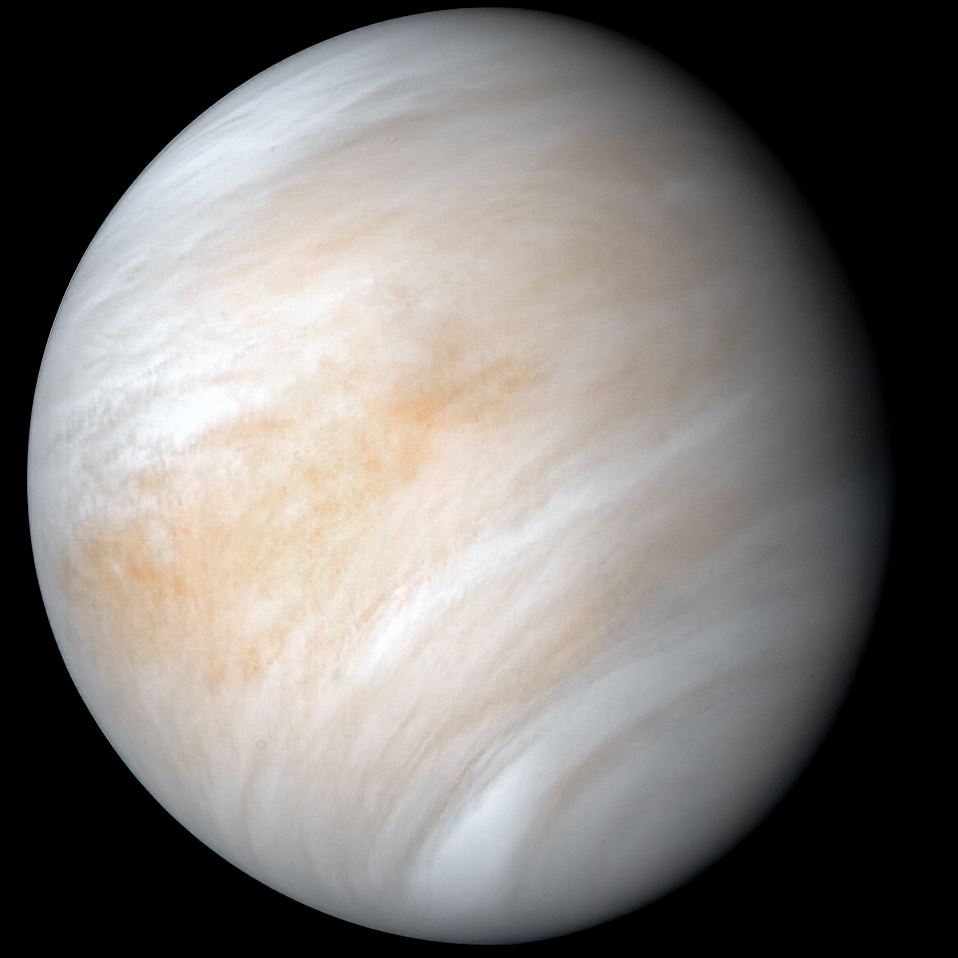
\includegraphics[width=\linewidth]{images/book1/g6-venus-mariner10.jpg}\\[2pt]
{\small 金星}
\end{minipage}\hfill
\begin{minipage}[t]{0.31\linewidth}\centering
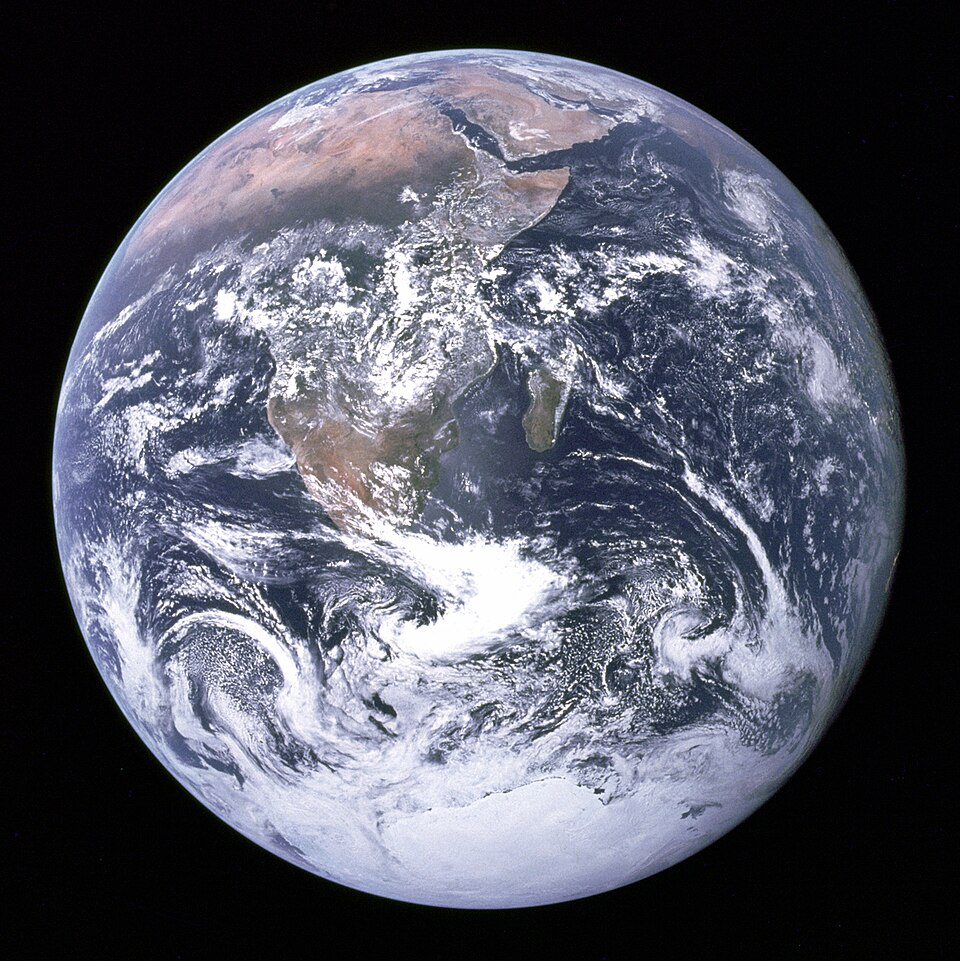
\includegraphics[width=\linewidth]{images/book1/g6-earth-apollo17.jpg}\\[2pt]
{\small 地球}
\end{minipage}\hfill
\begin{minipage}[t]{0.31\linewidth}\centering
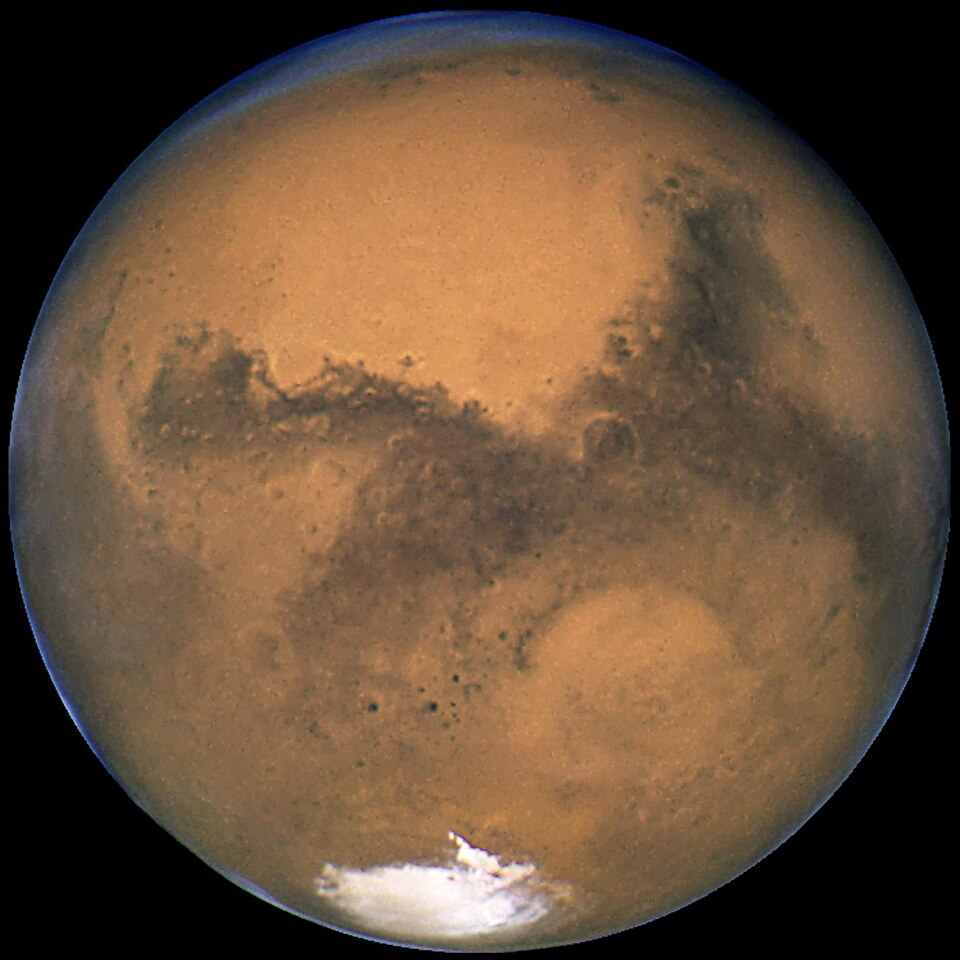
\includegraphics[width=\linewidth]{images/book1/g6-mars-hubble.jpg}\\[2pt]
{\small 火星}
\end{minipage}

\medskip
{\small 太空中的三张“明信片”。金星，由 Mariner~10
探测器于 1974 年拍摄，只能看到其\omterm{def:g4:clouds-rain-snow:cloud}{云层}顶部。地球，由 Apollo~17
机组成员在前往月球途中于 1972 年拍摄：非洲、阿拉伯半岛
以及白色\omterm{def:g4:clouds-rain-snow:cloud}{云层}下的\omterm{def:g3:continents-and-oceans:poles}{南极}洲冰雪。火星，由哈勃太空望远镜于 2003 年拍摄，
其极点处有一顶白色冰盖。
（照片：NASA/JPL-Caltech；NASA；NASA、ESA 和 Hubble Heritage Team。）}
% ledger: nasa:venus-mariner10, nasa:apollo17-earth, hubble:mars-2003
\end{omfigure}

\begin{recall}
物理教材已经说明：太阳是一颗恒星，是一个由炽热气体组成的巨大球体，
它能自身发光；行星是一种绕恒星运转的大型球状天体，
它自身不发光：我们之所以能看到它，是因为它反射
了恒星的光。太阳及绕它运行的一切天体构成
太阳系。每颗行星沿一条称为
轨道的路径绕太阳运行，并绕自转轴自转。我们周围的空气
压在它所接触的一切物体上：这就是气压。物质的密度
表示一定体积的该物质有多重：一立方厘米的水
重 1~克，所以其密度为 1~克每立方厘米；密度大于水的物质
会在水中下沉，密度较小的物质会漂浮。最后，约十分之七的
地球表面被\omterm{def:g2:water-on-earth:ocean}{海洋}覆盖
（见\cref{ch:g2:water-on-earth}）。
\end{recall}

\section{太阳周围的八颗行星}

八颗行星绕太阳运行。按照由近及远的顺序，
它们依次是水星、金星、地球、火星、木星、土星、
天王星和海王星。可用一句口诀帮助记忆这一顺序：\emph{水金地火木土天海
}（水星、金星、地球、火星、
木星、土星、天王星、海王星）。

下图按同一\omterm{def:g2:drawing-to-map:scale}{比例尺}并排画出八颗行星：
若一颗行星的宽度是另一颗的两倍，
则其圆的宽度也是两倍。

\begin{omfigure}
\pgfplotstableread{figdata/out/grade-6-planets-sizes.dat}\gsixsizes
\begin{tikzpicture}
  \draw[black!40] (-0.2,0) -- (13.8,0);
  \pgfplotstablegetrowsof{\gsixsizes}
  \pgfmathtruncatemacro{\gsixlast}{\pgfplotsretval-1}
  \foreach \i in {0,...,\gsixlast}{
    \pgfplotstablegetelem{\i}{x_cm}\of\gsixsizes \let\gx\pgfplotsretval
    \pgfplotstablegetelem{\i}{d_cm}\of\gsixsizes \let\gd\pgfplotsretval
    \pgfplotstablegetelem{\i}{name}\of\gsixsizes \let\gn\pgfplotsretval
    \pgfplotstablegetelem{\i}{d_km}\of\gsixsizes \let\gk\pgfplotsretval
    \pgfmathsetmacro{\gr}{\gd/2}
    \ifnum\i<4
      \fill[brown!70!black, draw=black!60, line width=0.3pt] (\gx,\gr) circle (\gr);
    \else
      \fill[orange!35, draw=black!60, line width=0.3pt] (\gx,\gr) circle (\gr);
    \fi
    \node[font=\scriptsize, rotate=40, anchor=north east, inner sep=1pt]
      at (\gx+0.08,-0.08) {\ifcase\i 水星\or 金星\or 地球\or 火星\or 木星\or 土星\or 天王星\or 海王星\fi};
  }
  \node[font=\scriptsize, align=left, anchor=north west] at (-0.2,4.15)
    {\tikz\fill[brown!70!black, draw=black!60] (0,0) circle (2.2pt); 岩质行星 \\
     \tikz\fill[orange!35, draw=black!60] (0,0) circle (2.2pt); 巨行星};
  \draw[|-|, black!70] (0,2.2) -- (1,2.2)
    node[midway, above, font=\scriptsize] {35\,000 千米};
\end{tikzpicture}

{\small 按比例画出的八颗行星（直径数据取自 NASA 行星
数据表）。行星之间的距离未按比例绘制：它们之间的距离太大，
一页纸根本无法容纳。}
% ledger: planet:Mercury.diameter, planet:Venus.diameter, planet:Earth.diameter, planet:Mars.diameter, planet:Jupiter.diameter, planet:Saturn.diameter, planet:Uranus.diameter, planet:Neptune.diameter (figdata/grade-6/planets.py, part sizes)
\end{omfigure}

前四颗离太阳最近的行星较小。接下来的四颗是\omterm{def:g6:earth-a-planet:planet-types}{巨行星}：
木星的宽度约为地球的 11 倍。那么太阳呢？按上图相同的比例绘制，
它将是一个约 40~厘米宽的圆盘
——比这一页纸还宽。
% ledger: planet:Jupiter.diameter, planet:Earth.diameter, sun:R (planets.py: sun_cm = 39.9 cm)

大小并非唯一的区别。下表给出了每颗行星的
直径、密度（单位为克每立方厘米）以及与太阳的
距离。

\begin{center}
\small
\begin{tabular}{lrrrr}
\hline
行星 & 直径（千米） & 密度（g/cm$^3$） & 与太阳的距离（百万千米）\\
\hline
水星 & 4\,879 & 5.4 & 58\\
金星 & 12\,104 & 5.2 & 108\\
地球 & 12\,756 & 5.5 & 150\\
火星 & 6\,792 & 3.9 & 228\\
\hline
木星 & 142\,984 & 1.3 & 779\\
土星 & 120\,536 & 0.7 & 1\,432\\
天王星 & 51\,118 & 1.3 & 2\,867\\
海王星 & 49\,528 & 1.6 & 4\,515\\
\hline
\end{tabular}
% ledger: planet:Mercury.diameter, planet:Venus.diameter, planet:Earth.diameter, planet:Mars.diameter, planet:Jupiter.diameter, planet:Saturn.diameter, planet:Uranus.diameter, planet:Neptune.diameter, planet:Mercury.density, planet:Venus.density, planet:Earth.density, planet:Mars.density, planet:Jupiter.density, planet:Saturn.density, planet:Uranus.density, planet:Neptune.density, planet:Mercury.dist, planet:Venus.dist, planet:Earth.dist, planet:Mars.dist, planet:Jupiter.dist, planet:Saturn.dist, planet:Uranus.dist, planet:Neptune.dist (figdata/grade-6/planets.py, main table)
\end{center}

密度把行星分成两类，两类之间没有过渡：
前四颗行星密度较大，超过 3.9~克每立方厘米，
与\omterm{def:g3:stones-pebbles-sand:rock}{岩石}和金属相近；后四颗行星密度较小，
低于 1.7~克每立方厘米。

\begin{definition}[岩质行星与巨行星]\label{def:g6:earth-a-planet:planet-types}
\emph{岩质行星}\index{岩质行星}是一类体积较小、密度较大的行星，
由\omterm{def:g3:stones-pebbles-sand:rock}{岩石}和金属构成，表面为固体，探测器可以在其上着陆：水星、金星、
地球和火星。\emph{巨行星}\index{巨行星}是一类体积很大、密度较小的行星，
主要由气体和液体构成，没有可供着陆的固体表面：
木星、土星、天王星和海王星。
% ledger: nasa:planet-families
\end{definition}

\begin{omfigure}
\begin{minipage}[c]{0.6\linewidth}\centering
\begin{tikzpicture}
  \begin{axis}[ybar, bar width=11pt, width=\linewidth, height=5.4cm,
      ymin=0, ymax=6.2, xmin=-0.6, xmax=7.6,
      xtick={0,...,7}, xticklabels={水星, 金星, 地球, 火星, 木星, 土星, 天王星, 海王星},
      xticklabel style={rotate=40, anchor=north east, font=\scriptsize},
      ytick={0,1,...,6}, ylabel={密度 (g/cm$^3$)},
      tick label style={font=\scriptsize}, label style={font=\scriptsize},
      axis x line*=bottom, axis y line*=left]
    \addplot[fill=brown!70!black, draw=black!60, bar shift=0pt, restrict x to domain=0:3]
      table[x=idx, y=density_gcm3] {figdata/out/grade-6-planets-density.dat};
    \addplot[fill=orange!35, draw=black!60, bar shift=0pt, restrict x to domain=4:7]
      table[x=idx, y=density_gcm3] {figdata/out/grade-6-planets-density.dat};
    \draw[blue!60!black, densely dashed] (axis cs:-0.6,1) -- (axis cs:7.6,1);
    \node[font=\scriptsize, blue!60!black, anchor=south, inner sep=1pt]
      at (axis cs:5,1) {水};
  \end{axis}
\end{tikzpicture}
\end{minipage}\hfill
\begin{minipage}[c]{0.36\linewidth}\centering
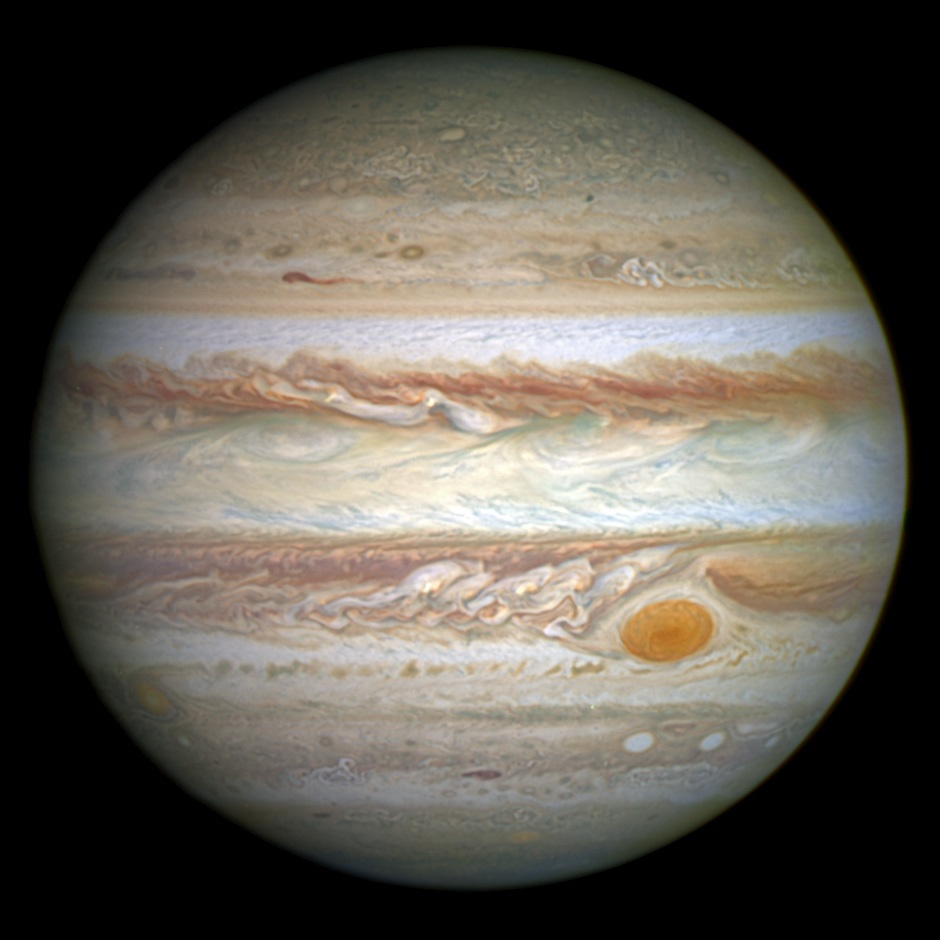
\includegraphics[width=0.9\linewidth]{images/book1/g6-jupiter-hubble.jpg}\\[2pt]
{\small 木星，哈勃太空望远镜于 2014 年拍摄。
（照片：NASA, ESA, A.~Simon。）}
% ledger: hubble:jupiter-2014
\end{minipage}

\smallskip
{\small 左图：八颗行星的密度，虚线表示
水的密度。右图：我们所看到的\omterm{def:g6:earth-a-planet:planet-types}{巨行星}，实际上是其
\omterm{def:g4:clouds-rain-snow:cloud}{云层}的顶部。}
% ledger: planet:Mercury.density, planet:Venus.density, planet:Earth.density, planet:Mars.density, planet:Jupiter.density, planet:Saturn.density, planet:Uranus.density, planet:Neptune.density (figdata/grade-6/planets.py, part density)
\end{omfigure}

木星照片中可以看到明暗相间的云带，以及一片红色的椭圆斑：
大红斑，一场比整个地球还大的\omterm{def:g5:natural-hazards:storm}{风暴}，
已经持续了数百年。\omterm{def:g4:clouds-rain-snow:cloud}{云层}之下没有地面，
只有气体，主要是氢和氦，
且越往深处越稠密。
% ledger: nasa:jupiter-gas

\begin{remark}[比水轻的行星]\label{rem:g6:earth-a-planet:saturn}
土星是唯一密度小于水的行星，
约为 0.7~克每立方厘米。若有一个足够大的浴缸，
能够容纳它，土星放进去就会漂浮！
% ledger: nasa:saturn-float, planet:Saturn.density
\end{remark}

\section{行星之间的距离有多远？}

行星不仅大小差别很大，彼此之间的距离
也非常遥远。地球距离太阳约 1.5 亿千米，
海王星是最远的行星，距离约为地球的 30 倍，
约 45 亿千米。下图将八颗行星按照与太阳的
实际距离，按比例画在同一条直线上。
% ledger: planet:Earth.dist, planet:Neptune.dist

\begin{omfigure}
\begin{tikzpicture}
  % whole system
  \draw[thick, gray] (0,0) -- (13.6,0);
  \fill[orange!80!yellow] (0,0) circle (3pt);
  \node[font=\scriptsize, above=3pt] at (0,0) {太阳};
  \foreach \n/\x/\lab in {Mercury/0.174/, Venus/0.326/, Earth/0.451/, Mars/0.687/,
                          Jupiter/2.345/木星, Saturn/4.313/土星, Uranus/8.636/天王星, Neptune/13.6/海王星} {
    \fill (\x,0) circle (1.4pt);
    \node[font=\scriptsize, above=3pt] at (\x,0) {\lab};
  }
  \draw[decorate, decoration={brace, amplitude=3pt, mirror}] (0.1,-0.25) -- (0.75,-0.25)
    node[midway, below=3pt, font=\scriptsize, align=center] {四颗 \\岩质行星};
  \draw[<->, thin, gray!70!black] (0,0.62) -- (13.6,0.62) node[midway, above, font=\scriptsize, black] {从太阳到海王星：约 45 亿千米};
  % the inner system, ten times larger
  \begin{scope}[yshift=-2.3cm]
    \draw[thick, gray] (0,0) -- (7.6,0);
    \fill[orange!80!yellow] (0,0) circle (3pt);
    \node[font=\scriptsize, above=3pt] at (0,0) {太阳};
    \foreach \n/\x in {水星/1.744, 金星/3.259, 地球/4.506, 火星/6.868} {
      \fill (\x,0) circle (1.4pt);
      \node[font=\scriptsize, below=3pt] at (\x,0) {\n};
    }
    \node[font=\scriptsize, anchor=west, align=left] at (8.0,0) {同一条直线，长度放大十倍，\\仅用于四颗岩质行星};
  \end{scope}
  \draw[dashed, gray] (0.75,-0.05) -- (7.6,-2.15);
\end{tikzpicture}

{\small 行星与太阳的距离，按比例绘制。上图：整个
太阳系，从太阳到海王星。下图：四颗\omterm{def:g6:earth-a-planet:planet-types}{岩质行星}，
放大十倍。图中圆点的大小不按比例绘制。}
% ledger: planet:Mercury.dist, planet:Venus.dist, planet:Earth.dist, planet:Mars.dist, planet:Jupiter.dist, planet:Saturn.dist, planet:Uranus.dist, planet:Neptune.dist (figdata/grade-6/planets.py, part dist)
\end{omfigure}

四颗\omterm{def:g6:earth-a-planet:planet-types}{岩质行星}都靠近太阳；四颗\omterm{def:g6:earth-a-planet:planet-types}{巨行星}则远在外侧，
彼此之间有很大的空隙。仅火星与木星之间的空隙就约为 5.5 亿千米，超过火星到太阳距离的两倍。
% ledger: planet:Mars.dist, planet:Jupiter.dist

要在同一比例下同时画出大小和距离很困难：行星
会变成看不见的小点。\emph{比例模型}可以帮助我们同时想象两者。

\begin{method}[制作太阳系的比例模型]\label{met:g6:earth-a-planet:scale-model}
\begin{enumerate}
  \item 选取模型中地球的大小，例如 1~厘米。
  \item 求模型中 1~厘米代表多少实际千米：用
        地球的实际直径（12\,756~千米）除以其在模型中的大小。
  \item 将每个实际大小和每个实际距离都除以这个数。
        然后把单位换成便于想象的单位（厘米、
        米、千米）。
\end{enumerate}
% ledger: planet:Earth.diameter
\end{method}

\begin{example}[地球是一颗弹珠]\label{ex:g6:earth-a-planet:marble}
若地球是一颗宽 1~厘米的弹珠，则 1~厘米代表 12\,756~千米。太阳
直径为 1\,391\,400~千米，在模型中变为一个宽 $1\,391\,400 \div 12\,756 \approx
109$~厘米宽的球，比一个小孩还高。地球距太阳
1.5 亿~千米：$149\,600\,000 \div 12\,756 \approx 11\,700$~厘米，
即约 117~米，相当于一个足球场的长度。
% ledger: planet:Earth.diameter, sun:R, planet:Earth.dist
\end{example}

\begin{center}\small
\begin{tabular}{|l|c|c|}
\hline
\textbf{天体} & \textbf{模型中的大小（厘米）} & \textbf{距太阳的距离（米）} \\
\hline
太阳 & 109 &——\\
水星 & 0.38 & 45 \\
金星 & 0.95 & 85 \\
地球 & 1.00 & 117 \\
火星 & 0.53 & 179 \\
木星 & 11.21 & 610 \\
土星 & 9.45 & 1123 \\
天王星 & 4.01 & 2248 \\
海王星 & 3.88 & 3540 \\
\hline
\end{tabular}
\end{center}
% ledger: sun:R, planet:Mercury.diameter, planet:Venus.diameter, planet:Earth.diameter, planet:Mars.diameter, planet:Jupiter.diameter, planet:Saturn.diameter, planet:Uranus.diameter, planet:Neptune.diameter, planet:Mercury.dist, planet:Venus.dist, planet:Earth.dist, planet:Mars.dist, planet:Jupiter.dist, planet:Saturn.dist, planet:Uranus.dist, planet:Neptune.dist (figdata/grade-6/planets.py, part model)

在这个模型中，直到海王星为止的整个太阳系铺展在一个
直径 7~千米的圆上，中央是一个大球，另有八个弹珠和
小球散落其上，其中最大的一个与柚子大小相当。
太阳系绝大部分是空旷的空间。

\section{金星、地球和火星}

金星、地球和火星是近邻，三者都是\omterm{def:g6:earth-a-planet:planet-types}{岩质行星}。金星
大小与地球几乎相同：其直径为地球的 95~\%。
火星较小：其直径约为地球的一半。然而这三颗
行星之间的差别却极大。
% ledger: planet:Venus.diameter, planet:Earth.diameter, planet:Mars.diameter (planets.py: 94.9 %)

\paragraph{金星。}金星被一层厚厚的大气包裹，这层大气主要由
二氧化碳构成，并伴有浓密的硫酸云，硫酸是一种腐蚀性很强的酸。其
大气如此厚重，对地面的压强是地球大气的 92~倍。
金星表面温度约为
464~$^\circ$C，热到足以熔化铅。那里
任何水都无法以液态存在。
% ledger: nasa:venus-clouds, planet:Venus.psurf, planet:Venus.Tmean

\paragraph{火星。}火星是一片寒冷、干燥、多尘的\omterm{def:g5:weather-and-climate:desert}{沙漠}。其大气
同样主要由二氧化碳组成，但非常稀薄：其对地面的压强
约为地球大气的百分之一。平均温度为
$-65$~$^\circ$C。如今那里仍可找到水，但以冰的形式存在：冰存在于
两极的极冠中，以及近极地区的地下。然而火星并非一直如此：
数十亿年前，火星上曾有\omterm{def:g1:landscapes-around-us:water}{河流}流过，形成\omterm{def:g1:landscapes-around-us:water}{湖泊}，
\omterm{def:g5:water-shapes-the-land:flood}{洪水}也曾席卷其表面。
% ledger: nasa:mars-water, planet:Mars.psurf, planet:Mars.Tmean

\paragraph{地球。}介于两者之间，地球大气对地面的压强
约为 1~巴（用来比较各行星大气压强的
单位），平均温度为 15~$^\circ$C，并拥有
由液态水构成的\omterm{def:g2:water-on-earth:ocean}{海洋}。
% ledger: planet:Earth.psurf, planet:Earth.Tmean

\begin{omfigure}
\begin{tikzpicture}[x=1cm, y=1cm,
    lab/.style={font=\scriptsize, align=center, text width=3.6cm},
    row/.style={font=\scriptsize\bfseries, anchor=east, align=right, text width=2.6cm}]
  % discs to scale: diameters 94.9 %, 100 %, 53.2 % of the Earth's (planets.py)
  \shade[ball color=yellow!60!orange!30] (3,0) circle (0.949);
  \shade[ball color=blue!55] (7,0) circle (1.0);
  \shade[ball color=red!55!brown] (11,0) circle (0.532);
  \node[font=\small\bfseries] at (3,-1.35) {金星};
  \node[font=\small\bfseries] at (7,-1.35) {地球};
  \node[font=\small\bfseries] at (11,-1.35) {火星};
  \foreach \y/\t in {-2.2/{压在地面上\\的空气}, -3.2/{平均\\温度},
                     -4.2/{表面的\\液态水}}
    {\node[row] at (1.1,\y) {\t};}
  \foreach \x in {3,7,11}{
    \foreach \y in {-2.2,-3.2,-4.2}{
      \draw[rounded corners=3pt, black!25, fill=black!3] (\x-1.8,\y-0.4) rectangle (\x+1.8,\y+0.4);}}
  \node[lab] at (3,-2.2) {\textbf{92 巴}\\压强极大};
  \node[lab] at (7,-2.2) {\textbf{1 巴}};
  \node[lab] at (11,-2.2) {\textbf{0.01 巴}\\极其稀薄};
  \node[lab, text=red!70!black] at (3,-3.2) {\textbf{464~$^\circ$C}};
  \node[lab] at (7,-3.2) {\textbf{15~$^\circ$C}};
  \node[lab, text=blue!60!black] at (11,-3.2) {\textbf{$-65$~$^\circ$C}};
  \node[lab] at (3,-4.2) {\textbf{否}\\太热};
  \node[lab, text=blue!60!black] at (7,-4.2) {\textbf{是}\\有海洋};
  \node[lab] at (11,-4.2) {\textbf{否}\\仅有冰};
\end{tikzpicture}

{\small 金星、地球和火星的比较。三个圆盘按
比例绘制。（数据来源：NASA 行星概况表。）}
% ledger: planet:Venus.psurf, planet:Earth.psurf, planet:Mars.psurf, planet:Mercury.Tmean, planet:Venus.Tmean, planet:Earth.Tmean, planet:Mars.Tmean, planet:Jupiter.Tmean, planet:Saturn.Tmean, planet:Uranus.Tmean, planet:Neptune.Tmean, nasa:mars-water
\end{omfigure}

\paragraph{冷与热。}离太阳近的行星接收到的
光和热很多；离太阳远的则很少。因此，行星离太阳越远，
就应越冷。下图表明，
从地球向外，此规律成立：远在外侧的\omterm{def:g6:earth-a-planet:planet-types}{巨行星}是冰冻的世界。
但看看金星：它离太阳的距离几乎是水星的两倍，
却更热！其厚重的二氧化碳大气像厚毯子一样
困住太阳的热量，不让它逸散。水星几乎没有大气，
留不住自身的热量。
% ledger: planet:Mercury.Tmean, planet:Venus.Tmean, planet:Earth.Tmean, planet:Mars.Tmean, planet:Jupiter.Tmean, planet:Saturn.Tmean, planet:Uranus.Tmean, planet:Neptune.Tmean, planet:Mercury.dist, planet:Venus.dist, planet:Earth.dist, planet:Mars.dist, planet:Jupiter.dist, planet:Saturn.dist, planet:Uranus.dist, planet:Neptune.dist, nasa:venus-clouds, planet:Mercury.psurf

\begin{omfigure}
\begin{tikzpicture}
  \begin{axis}[ybar, bar width=14pt, width=0.86\linewidth, height=6cm,
      ymin=-270, ymax=520, xmin=-0.6, xmax=7.6,
      xtick={0,...,7},
      xticklabels={{水星 \\58}, {金星 \\108}, {地球 \\150}, {火星 \\228},
                   {木星 \\779}, {土星 \\1432}, {天王星 \\2867}, {海王星 \\4515}},
      xticklabel style={align=center, font=\scriptsize},
      axis x line*=bottom, axis y line*=left,
      xticklabel pos=lower, ytick={-200,-100,...,500},
      ylabel={平均温度（$^\circ$C）}, xlabel={行星与太阳的距离（百万千米）},
      tick label style={font=\scriptsize}, label style={font=\scriptsize},
      nodes near coords, nodes near coords style={font=\tiny},
      every node near coord/.append style={/pgf/number format/1000 sep={}}]
    \addplot[fill=orange!50, draw=black!60, bar shift=0pt]
      table[x=idx, y=tmean_C] {figdata/out/grade-6-planets-temp.dat};
    \draw[black!50] (axis cs:-0.6,0) -- (axis cs:7.6,0);
  \end{axis}
\end{tikzpicture}

{\small 各行星的平均温度，按照与太阳的距离排列。
金星打破了这一规律：它比水星还热，而水星
离太阳更近。（数据来源：NASA 行星数据表。）}
% ledger: planet:Mercury.Tmean, planet:Venus.Tmean, planet:Earth.Tmean, planet:Mars.Tmean, planet:Jupiter.Tmean, planet:Saturn.Tmean, planet:Uranus.Tmean, planet:Neptune.Tmean, planet:Mercury.dist, planet:Venus.dist, planet:Earth.dist, planet:Mars.dist, planet:Jupiter.dist, planet:Saturn.dist, planet:Uranus.dist, planet:Neptune.dist (figdata/grade-6/planets.py, part temp)
\end{omfigure}

\section{是什么使地球适宜生命存在}

目前已知，地球是唯一存在生命的行星。生物
需要多种条件同时具备，而地球全部具备。

\begin{itemize}
  \item \textbf{液态水。}所有生物都需要液态水：地球
        上有\omterm{def:g2:water-on-earth:ocean}{海洋}、\omterm{def:g1:landscapes-around-us:water}{河流}和\omterm{def:g1:landscapes-around-us:water}{湖泊}。
  \item \textbf{温度适中。}在地表，水在 0~$^\circ$C 时凝固，
        在 100~$^\circ$C 时沸腾（物理）。地球平均温度为
        15~$^\circ$C，其温度大多
        介于两者之间，因此水保持液态。
  \item \textbf{距太阳的距离适中。}离太阳太近，像
        金星那样，行星有变得过热的风险；太远，像火星那样，
        则太冷。地球位于适合液态水存在的距离上。
  \item \textbf{大气。}包围地球的大气层使地表
        夜间保持温暖，为生物提供所需的气体，
        并对\omterm{def:g2:water-on-earth:ocean}{海洋}施加足够的压力，使水能保持液态。在
        火星上，空气极为稀薄，液态水难以长时间
        存在于地表：它会凝固，或化为蒸气。
\end{itemize}
% ledger: nasa:mars-water, planet:Earth.Tmean

\begin{remark}[火星上曾有生命吗？]\label{rem:g6:earth-a-planet:mars-life}
火星曾经有过\omterm{def:g1:landscapes-around-us:water}{河流}和\omterm{def:g1:landscapes-around-us:water}{湖泊}，科学家想知道微小的生物
是否曾在那里生存，即在很久以前，火星更温暖湿润的时候。
科学家并不指望今天的火星上存在生物；借助机器人
探测车，他们在\omterm{def:g3:stones-pebbles-sand:rock}{岩石}中寻找古代生命存在过的迹象。
% ledger: nasa:mars-water
\end{remark}

\section{从太空看地球}

几千年来，人们只能想象从外部看自己的星球
是什么样子。1968 年 12 月 24 日，阿波罗 8 号的宇航员
在绕月轨道上，看到地球从灰色的
月球地平线上升起，其中一人比尔·安德斯拍下了下图。
% ledger: nasa:earthrise

\begin{omfigure}
\begin{minipage}[c]{0.46\linewidth}\centering
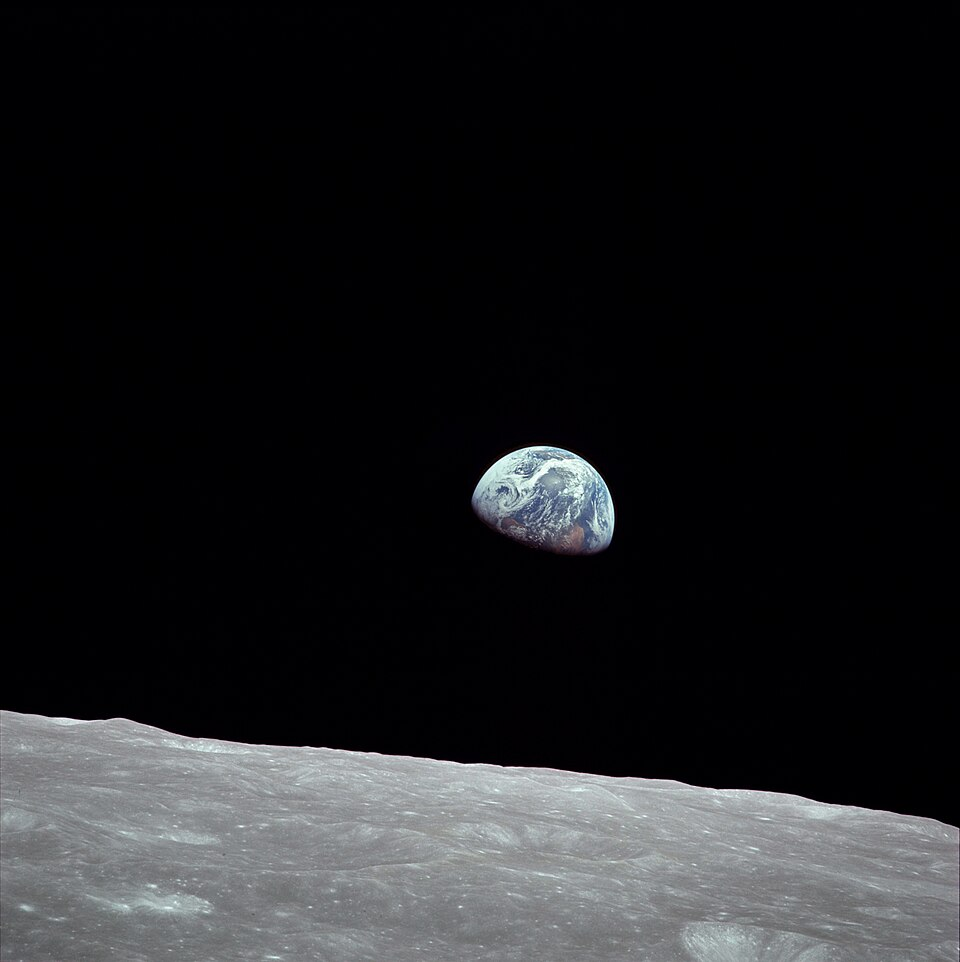
\includegraphics[width=0.85\linewidth]{images/book1/g6-earthrise.jpg}
\end{minipage}\hfill
\begin{minipage}[c]{0.5\linewidth}
{\small \emph{地球升起}：月球地平线上方的地球，
由绕月轨道上的阿波罗 8 号拍摄于 1968 年 12 月 24 日。
（照片：NASA，Bill Anders。）}

\medskip
{\small 请看颜色：\omterm{def:g2:water-on-earth:ocean}{海洋}的蓝、\omterm{def:g4:clouds-rain-snow:cloud}{云层}的白色漩涡、
陆地的棕色。四周是漆黑的太空，前景中是灰色而死寂的月面，
没有水，也没有
空气。}
\end{minipage}
% ledger: nasa:earthrise
\end{omfigure}

从太空看，地球大部分是蓝色的：\omterm{def:g2:water-on-earth:ocean}{海洋}覆盖着
约十分之七的表面。白色的水滴\omterm{def:g4:clouds-rain-snow:cloud}{云团}在上空翻卷，
两极覆盖着白色的冰。陆地干燥处呈棕色，
植物生长处呈绿色。空气本身看不见，但漂浮其中的云
说明它的存在。太阳系中的所有行星里，只有地球同时呈现这些颜色
：液态水、云和生长的植物。
% ledger: wss:ocean-cover, nasa:apollo17-earth

\begin{history}[暗淡蓝点]
\begin{minipage}[c]{0.66\linewidth}
1990 年 2 月 14 日，太空探测器旅行者 1 号距离太阳约 60 亿
千米，比海王星更远。在离开
太阳系之前，它将照相机转向身后，拍下了
地球的照片。照片中，我们的星球只是一个明亮的小点，
比一粒尘埃还小，悬浮在一束阳光中。天文学家卡尔·萨根
谈到它时写道：“再看一眼那个小点。那就是这里，那是
家园，那就是我们。”
% ledger: nasa:pale-blue-dot
\end{minipage}\hfill
\begin{minipage}[c]{0.3\linewidth}\centering
\begin{tikzpicture}
  \node[inner sep=0] (img) {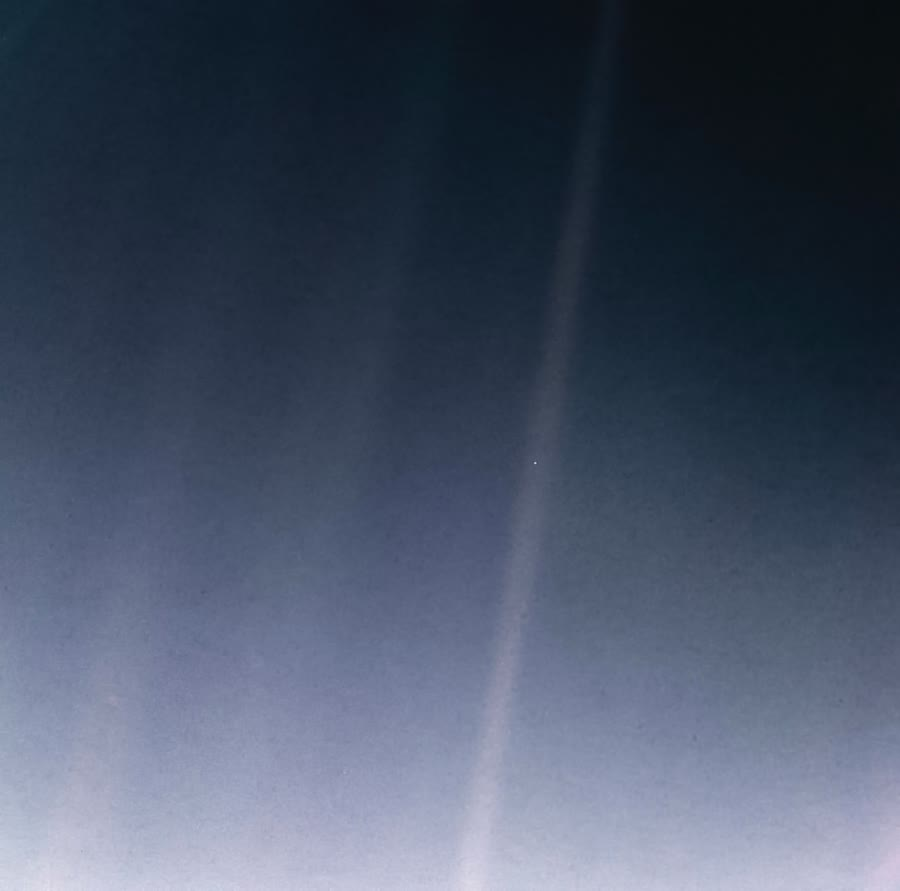
\includegraphics[width=\linewidth]{images/book1/g6-pale-blue-dot.jpg}};
  \draw[yellow!80!orange, thick] ($(img.south west)!0.594!(img.south east) + (0,{0.476*\linewidth})$) circle (6pt);
\end{tikzpicture}\\[2pt]
{\footnotesize 旅行者 1 号于 1990 年拍摄的地球（圈出处）。（图像：
NASA/JPL-Caltech，公有领域。）}
% ledger: nasa:pale-blue-dot
\end{minipage}
\end{history}

\section{练习}

\begin{exercise}[$\star$]\label{exo:g6:earth-a-planet:1}
按距离太阳由近到远的顺序，列出太阳系的八颗行星。
在\omterm{def:g6:earth-a-planet:planet-types}{岩质行星}下画横线。
\end{exercise}

\begin{exercise}[$\star$]\label{exo:g6:earth-a-planet:2}
抄写并补全：“\omterm{def:g6:earth-a-planet:planet-types}{岩质行星}体积小，\ldots{}，表面有固体
\ldots{}。\omterm{def:g6:earth-a-planet:planet-types}{巨行星}体积很大，\ldots{}较低，主要由
\ldots{}和\ldots{}”
\end{exercise}

\begin{exercise}[$\star$]\label{exo:g6:earth-a-planet:3}
利用本章的表格，哪颗行星的直径最接近
地球的直径？哪颗行星最大？哪颗行星最小？
\end{exercise}

\begin{exercise}[$\star$]\label{exo:g6:earth-a-planet:4}
判断下列说法是否正确，并改正错误的说法。
(a) 金星被\omterm{def:g2:water-on-earth:ocean}{海洋}覆盖。
(b) 火星比地球冷。
(c) \omterm{def:g6:earth-a-planet:planet-types}{巨行星}是离太阳最近的四颗行星。
(d) 土星的密度比水小。
\end{exercise}

\begin{exercise}[$\star\star$]\label{exo:g6:earth-a-planet:5}
水星的直径为 4\,879~千米，地球的直径为
12\,756~千米。求水星直径占地球直径的
百分比，结果四舍五入到整数。
% ledger: planet:Mercury.diameter, planet:Earth.diameter (planets.py: 38.2 %)
\end{exercise}

\begin{exercise}[$\star\star$]\label{exo:g6:earth-a-planet:6}
把地球一个挨一个排成一排，要横跨土星的直径
（120\,536~千米），需要多少个地球？结果四舍五入到整数。土星是\omterm{def:g6:earth-a-planet:planet-types}{岩质行星}
还是\omterm{def:g6:earth-a-planet:planet-types}{巨行星}？
% ledger: planet:Saturn.diameter, planet:Earth.diameter
\end{exercise}

\begin{exercise}[$\star\star$]\label{exo:g6:earth-a-planet:7}
天文学家在其他恒星周围发现了行星。行星~A 的密度为
1.1~克每立方厘米，直径是地球的 9 倍。
行星~B 的密度为 5.0~克每立方厘米，直径比地球略
小。哪一颗是\omterm{def:g6:earth-a-planet:planet-types}{岩质行星}，哪一颗是\omterm{def:g6:earth-a-planet:planet-types}{巨行星}？
请说明理由。
\end{exercise}

\begin{exercise}[$\star\star$]\label{exo:g6:earth-a-planet:8}
利用行星温度图：(a) 金星比地球高多少摄氏度？
(b) 火星比地球低多少
摄氏度？
% ledger: planet:Venus.Tmean, planet:Earth.Tmean, planet:Mars.Tmean
\end{exercise}

\begin{exercise}[$\star\star$]\label{exo:g6:earth-a-planet:9}
水星是离太阳最近的行星，但金星是最热的。请解释
原因。
\end{exercise}

\begin{exercise}[$\star\star$]\label{exo:g6:earth-a-planet:10}
地球距太阳 150~百万千米，火星距太阳 228~
百万千米。火星距太阳比地球远多少百万千米？
火星的距离比地球的距离大百分之几（结果
四舍五入到整数）？
% ledger: planet:Earth.dist, planet:Mars.dist
\end{exercise}

\begin{exercise}[$\star\star\star$]\label{exo:g6:earth-a-planet:11}
一位朋友说：“火星一直是干燥的\omterm{def:g5:weather-and-climate:desert}{沙漠}，那里从来没有
水。”请利用本章内容回答他：火星在数十亿年前
拥有什么，它的水今天在哪里，以及为什么液态水
现在不能在其表面存留？
\end{exercise}

\begin{exercise}[$\star\star\star$]\label{exo:g6:earth-a-planet:12}
金星有时被称为地球的孪生兄弟。它的直径为地球的 95~\%
，金星表面的重力为 8.9，而地球的为
9.8（同一标尺）。(a) 求金星表面重力占地球表面重力的
百分比，
结果四舍五入到整数。(b) 说出金星与地球
相像的两点，以及不相像的两点。
% ledger: planet:Venus.gravity, planet:Earth.gravity, planet:Venus.diameter
\end{exercise}

\section{问题：三颗行星的明信片}

\begin{problem}[{周末问题——三张来自太空的明信片，以及金星的大气
对地面施加多大的压力}]
\label{pb:g6:earth-a-planet:1}
% ledger: planet:Venus.dist, planet:Venus.diameter, planet:Venus.density, planet:Venus.Tmean, planet:Venus.psurf, planet:Earth.dist, planet:Earth.diameter, planet:Earth.density, planet:Earth.Tmean, planet:Earth.psurf, planet:Mars.dist, planet:Mars.diameter, planet:Mars.density, planet:Mars.Tmean, planet:Mars.psurf, nasa:venus-clouds, nasa:mars-water
三个机器人探测器各寄回一张明信片，
背面写着几个数字。

\begin{center}
\small
\begin{tabular}{>{\raggedright\arraybackslash}p{0.29\linewidth}>{\raggedright\arraybackslash}p{0.29\linewidth}>{\raggedright\arraybackslash}p{0.29\linewidth}}
\hline
\textbf{来自金星} & \textbf{来自地球} & \textbf{来自火星}\\
\hline
距太阳距离：108~百万千米。 & 距太阳距离：
150~百万千米。 & 距太阳距离：228~百万千米。\\
直径：12\,104~千米。 & 直径：12\,756~千米。 & 直径：6\,792~千米。\\
密度：5.2~g/cm$^3$。 & 密度：5.5~g/cm$^3$。 & 密度：3.9~g/cm$^3$。\\
平均温度：464~$^\circ$C。 & 平均温度：15~$^\circ$C。 &
平均温度：$-65$~$^\circ$C。\\
空气对地面的压强为 92~巴，厚厚的酸性\omterm{def:g4:clouds-rain-snow:cloud}{云层}。 &
空气对地面的压强为 1~巴，有\omterm{def:g2:water-on-earth:ocean}{海洋}和云。 &
空气对地面的压强为 0.01~巴，两极有冰。\\
\hline
\end{tabular}
\end{center}

\medskip
\noindent\textbf{第一部分——比较行星。}
\begin{enumerate}
  \item 将三颗行星按距太阳的远近排序。
  \item 金星比地球离太阳近多少百万千米？
        火星比地球离太阳远多少百万千米？
  \item 求火星直径占地球直径的百分比，
        结果取最接近的整数。火星宽度大约是地球的
        四分之一、一半还是四分之三？
  \item 这三颗行星是\omterm{def:g6:earth-a-planet:planet-types}{岩质行星}还是\omterm{def:g6:earth-a-planet:planet-types}{巨行星}？
        明信片上的哪些数据可以说明这一点？
\end{enumerate}

\medskip
\noindent\textbf{第二部分——大气。}
\begin{enumerate}[resume]
  \item 哪颗行星的大气最厚？
        哪颗行星的大气最薄？
  \item 火星大气对其地面的压强，是地球大气
        对地面压强的几分之一？
  \item 金星比地球离太阳近，但仅凭这一点无法解释
        464~$^\circ$C 的温度。金星的大气对太阳的热量
        起了什么作用？
  \item 金星大气对其地面的压强是地球上的多少倍？
        为什么着陆金星的探测器必须有非常坚固的外壳？
\end{enumerate}

\medskip
\noindent\textbf{第三部分——水与生命。}
\begin{enumerate}[resume]
  \item 在地球表面，水在 0~$^\circ$C 时凝固，在
        100~$^\circ$C 时沸腾。利用平均温度，解释为什么水
        在地球上呈液态。
  \item 若将一杯水放在金星的地面上，
        会发生什么？放在火星的地面上呢？
  \item 火星在数十亿年前曾有\omterm{def:g1:landscapes-around-us:water}{河流}和\omterm{def:g1:landscapes-around-us:water}{湖泊}。这说明
        与今天相比，火星在久远以前的\omterm{def:g5:weather-and-climate:climate}{气候}怎样？
  \item 在地球明信片的背面写下：用几句话
        给出地球上存在生命的四个原因。
\end{enumerate}
\end{problem}
